\documentclass[conference]{IEEEtran}

\usepackage{cite}
\usepackage{amsmath,amssymb,amsfonts}
\usepackage{graphicx}
\graphicspath{{../figures/}}
\usepackage{algorithm}
\usepackage{algpseudocode}
\usepackage{textcomp}
\usepackage{xcolor}
\usepackage{placeins}
\usepackage{booktabs}
\usepackage{url}
\usepackage[hidelinks]{hyperref}

\def\BibTeX{{\rm B\kern-.05em{\sc i\kern-.025em b}\kern-.08em
    T\kern-.1667em\lower.7ex\hbox{E}\kern-.125emX}}

\makeatletter
\def\ps@IEEEtitlepagestyle{%
\def\@oddhead{\normalfont\fontsize{7}{8}\selectfont
\begin{minipage}[t]{\textwidth}
\raggedright
2026 IEEE 3rd International Student Conference on Digital Generation\\
21--23 October, 2026, Astana, Kazakhstan
\end{minipage}\hfil}%
\let\@evenhead\@oddhead
\let\@oddfoot\@empty
\let\@evenfoot\@empty}
\makeatother

\begin{document}

\title{Design of a Multimodal Pipeline for Accessibility in E-Learning Content}

\author{}

\maketitle

\begin{abstract}
This paper presents the design of an algorithmic pipeline to improve accessibility in e-learning platforms. Online education format now is deeply integrated into higher education and becoming more common in primary and secondary education. With new possibilities new accessibility challenges were introduced. Most modern educational environments such as schools and universities provide only basic implementation of media player that complicates learning process for learners with hearing and visual impairments. We have implemented a unified multimodal pipeline prototype to generate accessibility supporting and reusable artifacts: automatic speech recognition (ASR) based word-level captions, visual context descriptions, and summaries. To prove its technical feasibility and viability, we conducted evaluation on bilingual corpus of 24 videos of various lengths and content types (12 English, 12 Russian, 3.29h total). Test corpus runs were conducted in two configurations: basic ASR-only (B0) and full multimodal preprocessing utilizing hosted large language model (LLM) service (B1). As a result, we obtained following metrics: B1 runs stayed below real-time factor (RTF)=1 for every video, with mean RTF=0.433 and B0 configuration runs resulted in mean RTF=0.193. Although ASR confidence is reported at mean value of 0.942, actual accuracy has not been manually evaluated during this research. The scene coverage of 91.7\% means temporal coverage of evaluated video span but does not reflect quality of covered information. Manual validation of caption accuracy and description quality is left for future work.
\end{abstract}

\begin{IEEEkeywords}
accessibility, e-learning, educational video, multimodal pipeline, automatic speech recognition, captioning, audio description
\end{IEEEkeywords}

\section{Introduction}
Integration of internet with education sphere advanced accessibility and eased education process generally, but pre-recorded lessons and screen-captured demonstrations are still unevenly accessible across student groups. Research on captions shows significant benefits for comprehension, attention and memory for various learner groups \cite{Gernsbacher2015}. More broadly, qualitative analysis of survey taken from neurodivergent, disabled and neurotypical students highlighted the accessibility support that recorded lessons provide, while captions and playback speed were especially important for disabled and neurodivergent students \cite{Horlin2024}. These accessibility features are often overlooked in educational environments and treated as separate products in commercials. Existing work on automatic adaptation of open educational resources (OER) proposes a methodology for adapting educational content to learner preferences utilizing AI to process and generate metadata for search and reuse \cite{IngavelezGuerra2022}. Our proposed approach combines word-level captions, scene descriptions and structured summaries into unified architecture. In this research we propose an engineering solution to advance accessibility: end-to-end pipeline that generates reusable synchronized artifacts. This framing is especially relevant in setup with compute limitation and application programming interface (API) request quotas. Research question - Can a multimodal processing pipeline generate reusable accessibility-supporting artifacts with practical processing latency on consumer-level hardware assisted by hosted models?

This paper contributes to:
\begin{enumerate}
\item Proof of technical feasibility of a unified multimodal processing pipeline with near-word-level accuracy, visual context description, and a structured summary per video.
\item Development of an adaptive scene indexing mechanism to keep temporal coverage high even in videos with very little scene differences.
\item Benchmarking on a balanced and normalized set of 24 educational videos in English and Russian.
\end{enumerate}

\section{Related Work}
\subsection{Captions and Learning Accessibility}
Related studies show that caption benefits spread beyond impaired learners; captions can also improve comprehension, attention, and recall of information \cite{Gernsbacher2015}. Additionally, automated subtitles can be beneficial under realistic conditions, but caption quality also heavily depends on temporal alignment and segmentation precision \cite{Malakul2023}. A study on synchronized captions adds that caption accuracy is insufficient without precise temporal alignment \cite{Mirzaei2018}. W3C media-accessibility guidance also requires synchronized captions, content descriptions, playback control, and navigation to fit modern accessibility standards \cite{W3CMediaReqs}. But still, modern solutions mostly implement captions as isolated features rather than integrated artifacts with multimodal support.

\subsection{Cognitive Load \& Neurodiversity in Video Based Education}
Existing studies on educational videos show that pacing, media intelligibility, segmentation, and learner control are key conditions for video-based education effectiveness \cite{Lange2020}. The absence of these conditions is a barrier that can affect engagement and comprehension \cite{Lange2020}. For disabled and neurodivergent students, recorded lessons are especially valuable if a framework allows flexible control over learning pace through playback control and captions \cite{Horlin2024}. Moreover, research on neurodivergent learners supports the claim that transcript errors, unclear navigation and overloaded presentation of content can complicate video-based learning for neurodivergent students \cite{LeCunff2024}. However, these studies discuss learning needs and media design nuances, while less attention is given to automatic generation of accessibility-supporting artifacts from educational video.

\subsection{Automatic Speech Recognition and Timestamping}
Modern automatic speech recognition (ASR) systems have reached practical use through deep-learning pipelines \cite{Malik2020} and large-scale weakly supervised models such as Whisper \cite{Radford2022}. Augmented methods such as WhisperX and CrisperWhisper target timestamp precision using forced alignment and attention-based refinement \cite{Bain2023,Wagner2024}. In the current prototype, ASR and timestamping mainly serve the caption artifact layer: they provide synchronized text that the player and downstream pipeline layers can reuse.

\subsection{Visual Accessibility and Audio Description}
Prior work on scene description authoring proposes evaluation of quality of descriptions by objectivity, succinctness, sufficiency, accuracy, referability, and clarity \cite{Natalie2021}.
In our prototype, scene-linked descriptions are presented as optional on-demand activation feature with spoken output within the processing pipeline rather than pre-rendered into source media file. In current research, the focus is on system integration and timing evaluation, but not user-study evaluation of description quality.

\section{System Design}
\subsection{Pipeline Architecture and Artifacts}
The implemented pipeline follows hybrid multimodal architecture, employing hosted multimodal LLM for complex visual context recognition while running compute-light deterministic algorithms for processing of large volume of media on owned server or locally in our case. To improve performance on consumer-grade hardware, the audio and visual branches execute concurrently.
As result of pre-processing stage, the system outputs three artifact groups:
\begin{itemize}
\item \textbf{Subtitle artifacts} ($A_{sub}$): near word-level timestamps, segment timing, and Web Video Text Tracks.
\item \textbf{Scene artifacts} ($A_{scene}$): time-indexed scenes list with textual descriptions.
\item \textbf{Structure artifacts} ($A_{sum}$): summary points and chapter markers extracted from scene descriptions.
\end{itemize}

\begin{figure*}[!t]
\centering
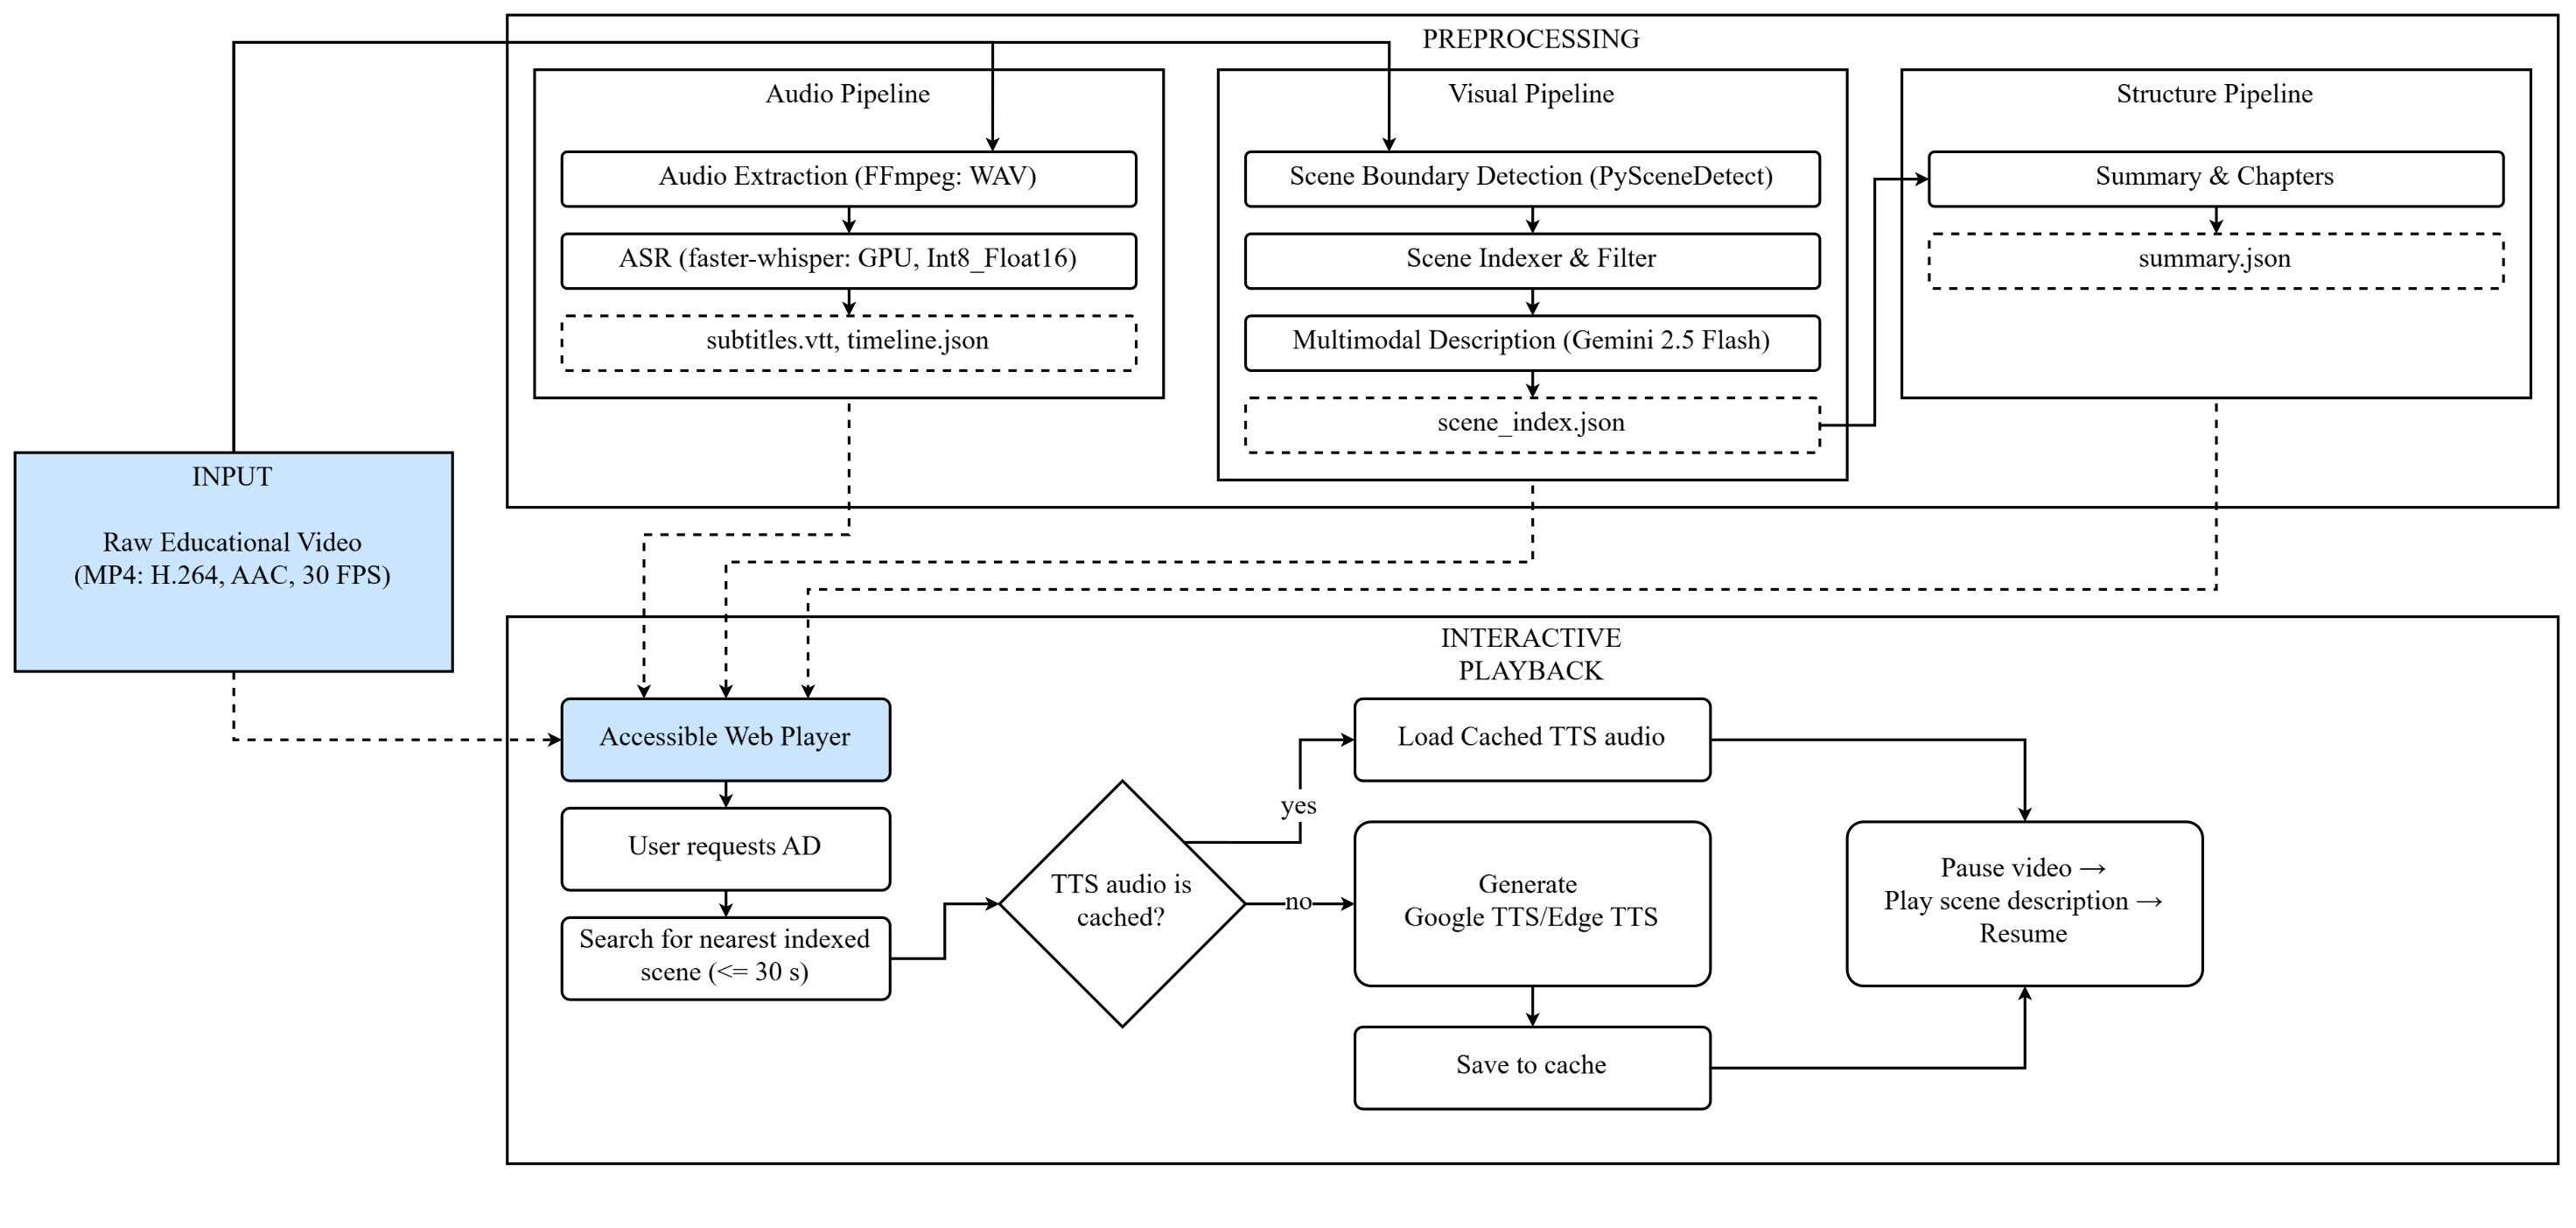
\includegraphics[width=0.95\textwidth]{fig_pipeline_arch.drawio.png}
\caption{Unified accessibility pipeline architecture. Offline preprocessing generates reusable artifacts; during playback, audio description is requested on demand and cached for subsequent calls.}
\label{fig:architecture}
\end{figure*}

\subsection{Interaction Layer and Artifact Rendering}
To implement per-word highlighting, we used a midpoint-based word grouper which is intended to stabilize the word selection and avoid temporal overlap. Though the evaluated corpus has not shown subtitle overlapping errors across adjacent words, this does not guarantee that an overlapping error will not occur in other cases. We implemented custom web media player and subtitle renderer with customizable font, contrast and word highlighting settings, because native HTML \texttt{<track>} elements do not fulfill the requirements selected for the current prototype such as stateful word-by-word highlighting, including current, previous, and upcoming states. The custom player looks for the nearest indexed scene within 15-seconds radius threshold, then returns cached audio when available or calls a text-to-speech (TTS) service to synthesize speech from the stored description and caches it. Implemented on demand spoken out description feature works as shown in Algorithm~\ref{alg:ad}.

\begin{algorithm}[!t]
\caption{On-Demand Audio Description Resolution}
\label{alg:ad}
\begin{algorithmic}[1]
\Require $T_{\text{req}}$ (current playback time in seconds)
\Require $I_{\text{scene}}$ (array of indexed scenes)
\Require $L_{\text{req}}$ (requested speech language)
\State $S_{\text{nearest}} \gets \text{select\_nearest}(I_{\text{scene}}, T_{\text{req}})$
\If{$|S_{\text{nearest}}.time - T_{\text{req}}| > 15.0$}
    \State \Return \text{Error (No scene nearby)}
\EndIf
\State $CacheKey \gets (S_{\text{nearest}}.id, L_{\text{req}})$
\If{\text{exists}($CacheKey$)}
    \State $Audio \gets \text{read\_cache}(CacheKey)$
\Else
    \If{\text{google\_tts\_available}()}
        \State $Audio \gets \text{synthesize\_preferred}(S_{\text{nearest}}.desc, L_{\text{req}})$
    \Else
        \State $Audio \gets \text{synthesize\_fallback}(S_{\text{nearest}}.desc, L_{\text{req}})$
    \EndIf
    \State $\text{write\_cache}(CacheKey, Audio)$
\EndIf
\State $\text{pause\_video}()$
\State $\text{play\_audio}(Audio)$
\State $\text{resume\_video}()$
\State \Return $Audio$
\end{algorithmic}
\end{algorithm}

\section{Methodology}
\subsection{Prototype Configuration}
The current prototype implementation focuses on Russian and English language support and instantiates the architecture described in Fig.~\ref{fig:architecture} with the following components:
\begin{enumerate}
\item \textbf{Transcribing:} the system uses a Whisper model optimized for the \texttt{int8\_float16} compute type \cite{Radford2022}. This provides a balance between transcription accuracy and real-time factor (RTF).
\item \textbf{Visual Semantic Extraction:} Visual transitions are detected with PySceneDetect and a predefined pixel-difference threshold \cite{PySceneDetect}. In the next step, the system calls the hosted \texttt{gemini-2.5-flash} multimodal model \cite{GeminiTeam2025} to generate a semantic description that captures textual and structural visual data from each identified scene.
\item \textbf{Adaptive Scene Indexing:} Because heuristic detection occasionally falls short on visually static content such as screencasts, we handle these low-variance scenarios by falling back to \emph{Adaptive Uniform Sampling}. This guarantees a baseline density of at least two descriptions per minute.
\end{enumerate}

\section{Technical Evaluation}
\subsection{Experimental Design and Corpus}
We evaluated the pipeline using a \emph{Bilingual Multimodal Corpus Benchmark} containing 24 educational videos (197.61 minutes in total): 12 videos in English and 12 in Russian. For both languages, we selected educational videos of various durations (short: 21.18 min, medium: 51.71 min, long: 124.73 min) and content types (talking-head, slide-centric, screencast, and practical demo). The test video corpus was assembled from mixed educational sources and further normalized to 1280$\times$720 at 30 frames per second (FPS). The corpus manifest preserves neither detailed source provenance nor license metadata, so the corpus should be treated as an internal engineering benchmark. Processing was conducted on a local workstation (AMD Ryzen 9 5900HX, NVIDIA RTX 3050 Notebook, 16 GB of RAM) to establish a baseline for consumer-grade deployability.

\begin{table}[t]
\caption{Corpus Composition}
\label{tab:corpus_comp}
\centering
\footnotesize
\setlength{\tabcolsep}{5pt}
\begin{tabular}{lccc}
\toprule
\textbf{Language} & \textbf{Short} & \textbf{Medium} & \textbf{Long} \\
\midrule
English & 4 & 4 & 4 \\
Russian & 4 & 4 & 4 \\
\bottomrule
\end{tabular}
\end{table}

Two configurations were compared:
\begin{itemize}
\item \textbf{B0 (ASR-only):} transcript and subtitle artifacts without visual branch.
\item \textbf{B1 (Full):} ASR + visual scene indexing + multimodal descriptions + summary/chapter generation.
\end{itemize}
The chosen configurations characterize pre-playback artifact generation. User-triggered text-to-speech calls are not included in the full-run timing because they depend on the network, and the current user-grade test workstation is not sufficient for running a local multimodal LLM comparable to \texttt{gemini-2.5-flash}.

\begin{table}[t]
\caption{Key Experimental Parameters}
\label{tab:exp_params}
\centering
\footnotesize
\setlength{\tabcolsep}{4.5pt}
\begin{tabular}{ll}
\toprule
\textbf{Component} & \textbf{Setting} \\
\midrule
ASR model & faster-whisper medium \\
ASR compute type & int8\_float16 (GPU) \\
Scene detector & PySceneDetect ContentDetector \\
Scene threshold & 27 \\
Scene indexing & Adaptive density (no static cap) \\
Description stage & Hosted multimodal API \\
TTS (interactive path) & Google Cloud Neural TTS (edge-tts fallback) \\
Pipeline mode & On-demand audio description \\
\bottomrule
\end{tabular}
\end{table}

\subsection{Evaluation Metrics}
This paper reports engineering proxy metrics, not direct measures of improved learning or accessibility effectiveness:
\begin{equation}
\text{low\_conf\_ratio} = \frac{w_{<0.5}}{w_{\text{all}}}
\end{equation}
\begin{equation}
\text{coverage}_{15s} = \frac{s_{\text{covered}}}{s_{\text{video}}}
\end{equation}
\begin{equation}
\text{RTF} = \frac{T_{\text{processing}}}{T_{\text{video}}}
\end{equation}
where RTF $< 1$ means preprocessing faster than the video duration. For implementation, the denominators for both RTF and coverage are derived from the same effective video span: the end time of the generated timeline for each video. Thus, $T_{\text{video}}$ denotes the scalar duration used for RTF, while $s_{\text{video}}$ denotes the length of the evaluated timeline span used for coverage. This keeps B0/B1 denominators consistent for each video. In this definition, $T_{\text{processing}}$ includes pre-playback processing stages only; RTF is therefore interpreted as batch preprocessing throughput rather than end-to-end playback latency. ASR confidence is an internal diagnostic of the Whisper model. Since no manual transcription accuracy checks, such as word error rate (WER) and character error rate (CER), were conducted, the metrics should not be interpreted as proof of transcription accuracy. The $\text{coverage}_{15s}$ metric shows the proportion of the evaluated video span covered by at least one scene anchor within a radius of 15 seconds. The 15-second radius was selected as half of the 30-second uniform grid used in the post hoc ablation. This metric does not indicate whether the generated description is sufficient or useful.

Additional diagnostics characterize alignment stability and visual indexing behavior:
\begin{equation}
\text{overlap\_ratio} = \frac{n_{\text{overlap}}}{\max(w_{\text{all}}-1,1)}
\end{equation}
\begin{equation}
\text{scene\_density} = \frac{n_{\text{scene}}}{T_{\text{video}}/60}
\end{equation}
\begin{equation}
\text{tail\_uncovered} = \max(0, T_{\text{video}} - t_{\text{last\_scene}})
\end{equation}
where $n_{\text{overlap}}$ is the number of overlapping adjacent word timestamps, and $t_{\text{last\_scene}}$ is the timestamp of the final indexed scene.

\subsection{Automation and Reproducibility}
All runs are conducted via a single driver script, which reads the corpus manifest and processes every video consecutively in B0 and B1 configurations. For single-video processing, the system applies a multithreaded pipeline scheme to reduce the total runtime. The driver saves pipeline output artifacts and computes summaries and metrics in machine-readable format, including baseline comparisons and a JavaScript Object Notation (JSON) report for further analysis. Tables and figures in this paper that are related to metrics are based on the 24-video corpus. The system rejects runs before tables and summary metrics are generated by checking for non-positive runtimes, missing rows, and out-of-range coverage values. If valid artifacts already exist for the current configuration, the driver reuses them, which supports the cache-aware design of the pipeline. However, hosted model calls can return different results depending on model patches, network conditions, and the probabilistic behavior of LLM-based services.

\subsection{Post Hoc Scene Selection Ablation}
We conducted post-hoc scene selection ablation on a frozen evaluation snapshot. The same cached B1 scene timestamps were reused without rerunning the pipeline. We compared fixed caps of 10, 20 and 30 scenes with uniform 60 s and 30 s grids and recomputed the same within-15 s coverage metric. These comparisons are coverage-oriented diagnostics of scene-selection policy, not alternative semantic scene detection methods.

\subsection{Qualitative Case Selection}
In addition to the aggregate metrics, we selected four artifact sets from cached B1 outputs: the lowest coverage case, a screencast reference, the densest practical demo, and a talking-head reference. These cases are used exclusively for surface-level checks and do not serve as evidence of semantic correctness or accessibility impact for real users. Selected cases are presented in the results section to link aggregate metrics with specific failure modes and design implications.

\FloatBarrier
\section{Results and Analysis}
\subsection{Aggregate Performance}
Table~\ref{tab:lang_overall} shows language-level and overall aggregates. The ASR component remains stable across languages (overall confidence mean 0.942 and low-confidence ratio mean 0.026). Baseline B0 is consistently fast (overall mean RTF 0.193), while B1 adds overhead but remains practical (overall mean 0.433, median 0.424).

\begin{table}[t]
\caption{Aggregate Results by Language and Overall}
\label{tab:lang_overall}
\centering
\footnotesize
\setlength{\tabcolsep}{4.2pt}
\begin{tabular}{lcccccc}
\toprule
\textbf{Scope} & \textbf{N} & \textbf{B0} & \textbf{B1} & \textbf{B1} & \textbf{ASR} & \textbf{Cov.} \\
 &  & \textbf{RTF}\textsubscript{mean} & \textbf{RTF}\textsubscript{mean} & \textbf{RTF}\textsubscript{med} & \textbf{conf.} & \textbf{15s} \\
\midrule
EN & 12 & 0.158 & 0.369 & 0.353 & 0.948 & 91.58\% \\
RU & 12 & 0.228 & 0.497 & 0.504 & 0.937 & 91.82\% \\
Overall & 24 & 0.193 & 0.433 & 0.424 & 0.942 & 91.70\% \\
\bottomrule
\end{tabular}
\end{table}

\subsection{Baseline Overhead and Throughput Behavior}
Table~\ref{tab:duration_baseline} compares B0/B1 across short, medium, and long videos. When comparing B0 mean RTF to B1 mean RTF, the highest overhead ratio is observed in the short-video set. Table~\ref{tab:stage_latency} shows the split of absolute processing time (seconds) between the audio-only pipeline (B0) and visual semantic extraction overhead. The overhead increases with both scene count and video duration.

\begin{table}[t]
\caption{Stage-Level Latency Breakdown (Mean Seconds)}
\label{tab:stage_latency}
\centering
\footnotesize
\setlength{\tabcolsep}{5pt}
\begin{tabular}{lccc}
\toprule
\textbf{Duration} & \textbf{Audio Pipeline} & \textbf{Visual Overhead} & \textbf{Total (B1)} \\
\midrule
Short & 28.8 & 49.0 & 77.7 \\
Medium & 69.4 & 74.2 & 143.6 \\
Long & 191.6 & 193.6 & 385.3 \\
\bottomrule
\end{tabular}
\end{table}

\begin{table}[t]
\caption{Baseline Comparison by Duration Bucket}
\label{tab:duration_baseline}
\centering
\footnotesize
\setlength{\tabcolsep}{4.2pt}
\begin{tabular}{lcccc}
\toprule
\textbf{Duration} & \textbf{N} & \textbf{B0 RTF}\textsubscript{mean} & \textbf{B1 RTF}\textsubscript{mean} & \textbf{B1/B0} \\
\midrule
Short & 8 & 0.192 & 0.522 & 2.71$\times$ \\
Medium & 8 & 0.178 & 0.365 & 2.05$\times$ \\
Long & 8 & 0.208 & 0.414 & 1.99$\times$ \\
Overall & 24 & 0.193 & 0.433 & 2.25$\times$ \\
\bottomrule
\end{tabular}
\end{table}

Fig.~\ref{fig:rtf} visualizes B0 and B1 RTF across content types using boxplots. Full pipeline processing remains below real-time for all 24 videos in the corpus.

\begin{figure}[!t]
\centering
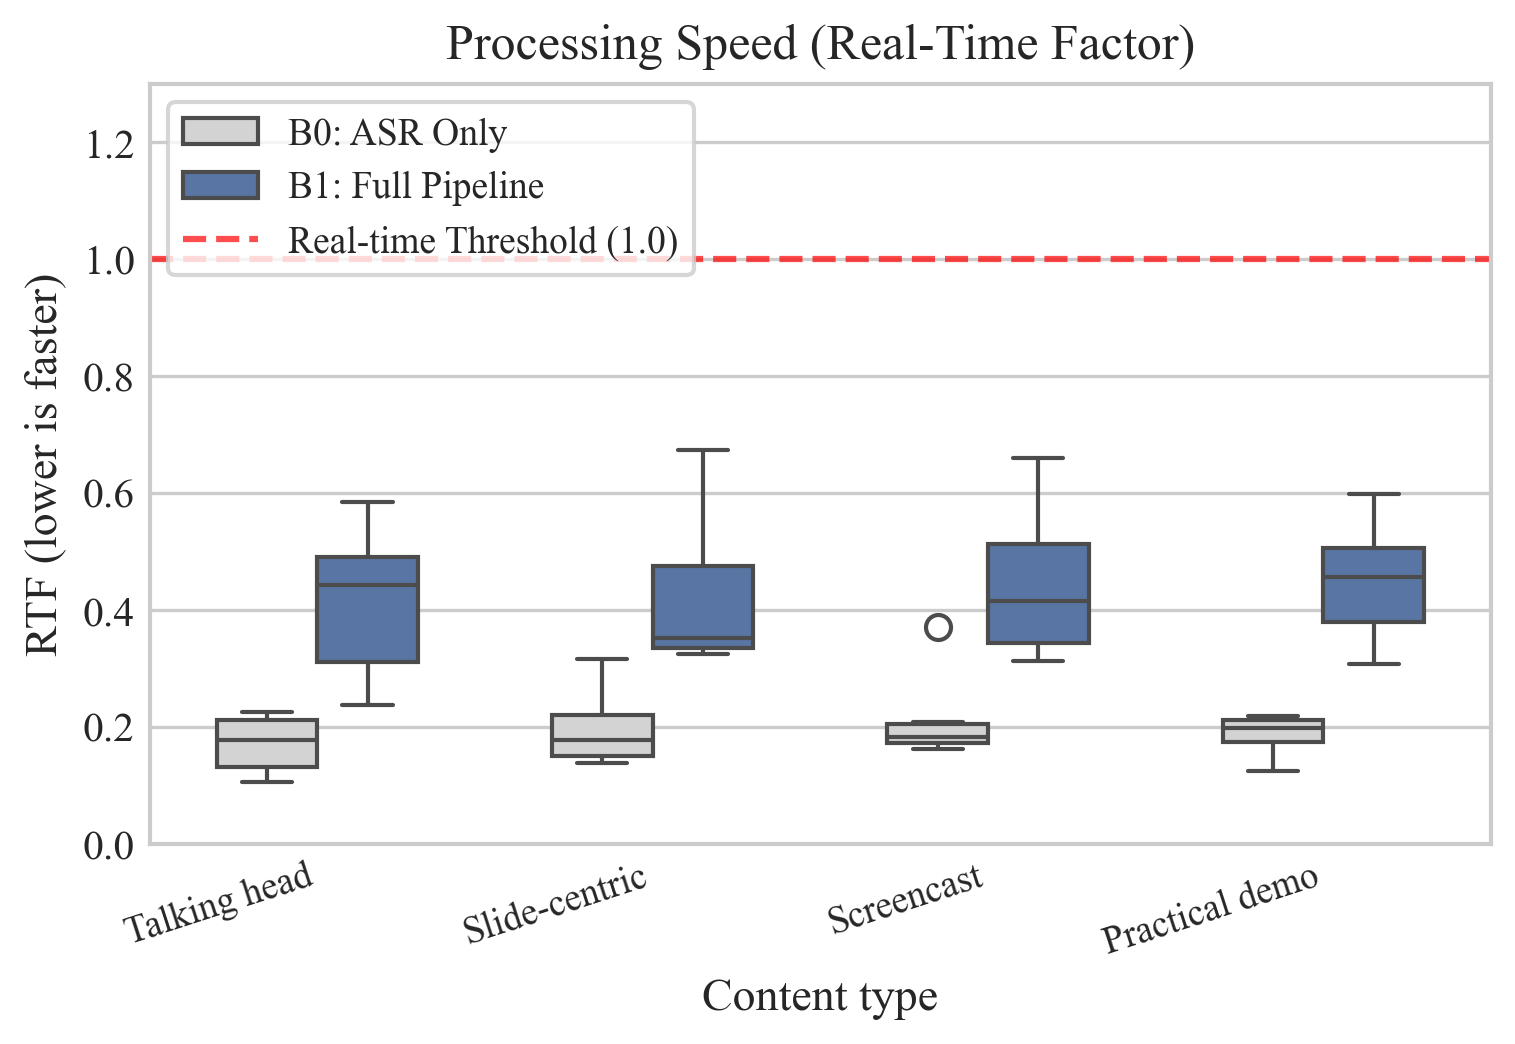
\includegraphics[width=\columnwidth]{fig_rtf_comparison.png}
\caption{Processing Speed (Real-Time Factor) across content types. The box spans the interquartile range (IQR), the horizontal line marks the median, and the whiskers denote the rest of the distribution up to $1.5 \times \text{IQR}$. A lower RTF indicates faster processing (the red dashed line represents real-time RTF=1.0).}
\label{fig:rtf}
\end{figure}

\subsection{Failure Cases and Practical Constraints}
Coverage variation is driven by visual characteristics. Low-variance screencasts remain a stress case for motion-based scene detection, so the pipeline applies fallback sampling when heuristic triggers are sparse. In the evaluated corpus, this kept screencast mean coverage at 94.58\%, while the overall mean coverage reached 91.7\%. Fig.~\ref{fig:coverage} shows the resulting content-type coverage distribution; the error bars summarize uncertainty within each six-video content-type group.

\begin{table}[t]
\caption{Content-Type Sensitivity (B1)}
\label{tab:content_sensitivity}
\centering
\footnotesize
\setlength{\tabcolsep}{4.2pt}
\begin{tabular}{lccccc}
\toprule
\textbf{Content type} & \textbf{N} & \textbf{B1 RTF} & \textbf{Cov. 15s} & \textbf{Scenes} & \textbf{Zero} \\
 &  & \textbf{mean} & \textbf{mean} & \textbf{mean} & \textbf{scene} \\
\midrule
Talking-head & 6 & 0.414 & 90.37\% & 29.83 & 0 \\
Slide-centric & 6 & 0.425 & 87.28\% & 33.67 & 0 \\
Screencast & 6 & 0.445 & 94.58\% & 39.00 & 0 \\
Practical demo & 6 & 0.449 & 94.55\% & 51.83 & 0 \\
\bottomrule
\end{tabular}
\end{table}

According to the results presented in Table~\ref{tab:content_sensitivity}, screencast-type content appears to have the highest overall coverage when fallback sampling is used, while slide-centric content shows the lowest mean coverage, presumably because of rare slide transitions, which are typical for this type of content. Practical demos are the most saturated in terms of the mean detected scene count. All content types achieved coverage above 87\%.

\begin{table}[t]
\caption{Post Hoc Scene Selection Ablation}
\label{tab:scene_ablation}
\centering
\footnotesize
\setlength{\tabcolsep}{5pt}
\begin{tabular}{lcc}
\toprule
\textbf{Strategy} & \textbf{Scenes} & \textbf{Cov. 15s} \\
 & \textbf{mean} & \textbf{mean} \\
\midrule
Adaptive index & 38.58 & 91.69\% \\
Static cap 10 & 9.71 & 63.79\% \\
Static cap 20 & 16.62 & 80.25\% \\
Static cap 30 & 21.58 & 87.18\% \\
Uniform 60 s & 8.62 & 51.07\% \\
Uniform 30 s & 16.75 & 98.74\% \\
\bottomrule
\end{tabular}
\end{table}

Table~\ref{tab:scene_ablation} presents a trade-off comparison with ablation outcomes. Adaptive scene indexing shows the highest mean scene count (38.58 scenes) and the second-highest mean temporal coverage. Post-hoc caps of 10, 20, and 30 scenes produced mean coverage values of 63.79\%, 80.25\%, and 87.18\%, respectively. A uniform 30 s interval achieved 98.74\% mean coverage because of the 15 s coverage radius, but this does not imply any quality improvement. Following cases illustrate why coverage metric should be considered along with content type. The coverage-wise weakest case (\texttt{ru\_medium\_slide-centric}) reached 48.0\% coverage with 8 scenes and maximum of 143.20 seconds interval between neighboring scene anchors, which is typical of slide-centric content. On the other hand, \texttt{en\_short\_screencast} resulted in 94.8\% with 12 scenes, and \texttt{en\_long\_practical\_demo} reached 100.0\% with 123 scenes across about 1184 seconds of source video.

\begin{figure}[!t]
\centering
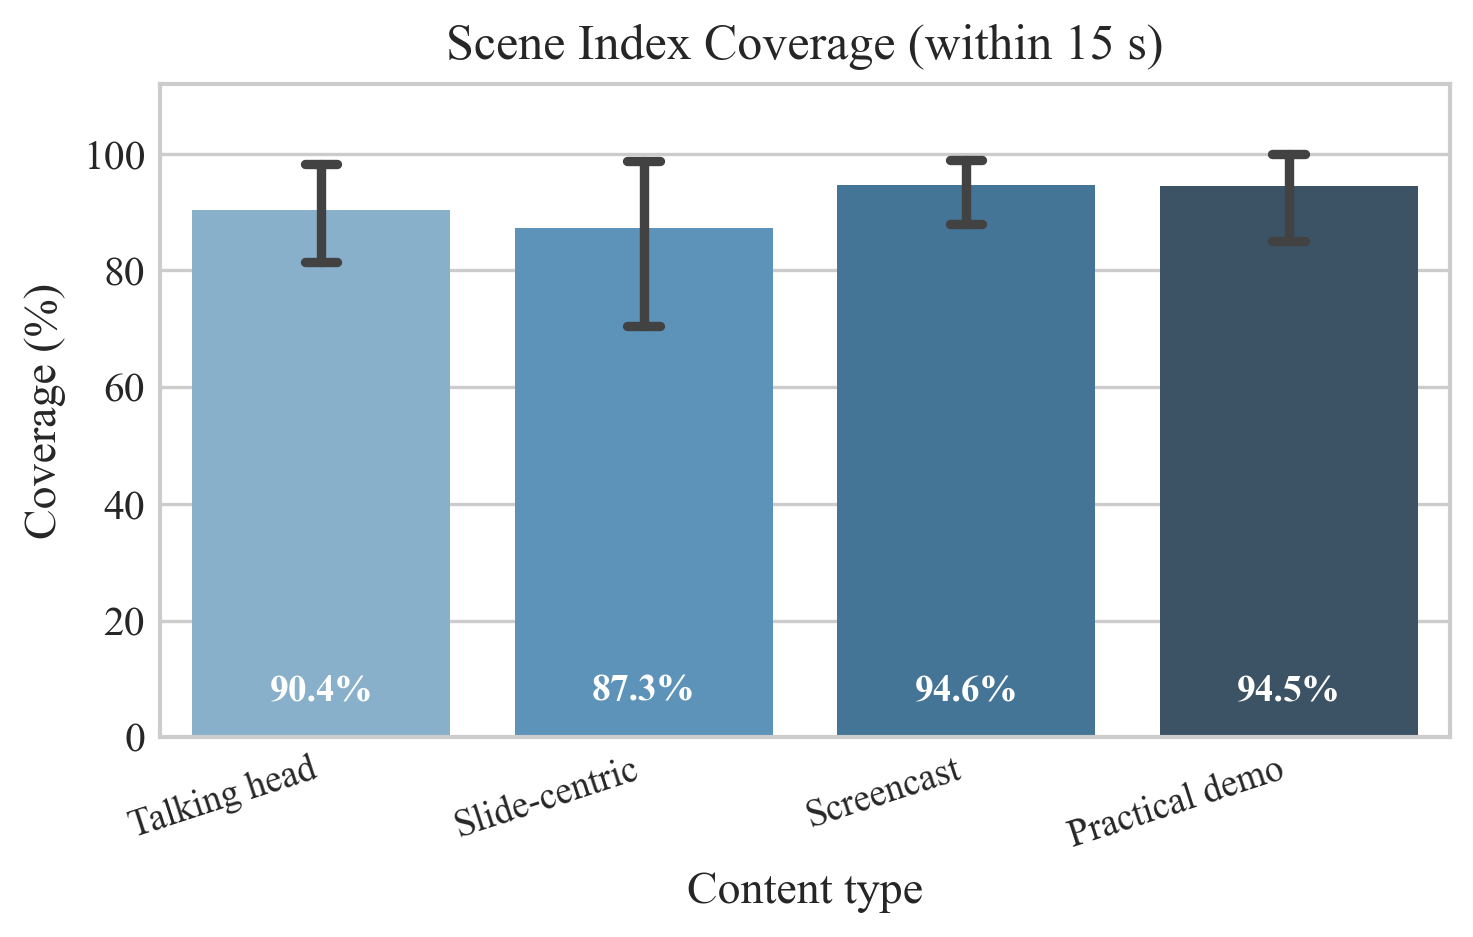
\includegraphics[width=\columnwidth]{fig_coverage.png}
\caption{Mean coverage within 15 s of indexed scenes by content type. Error bars show bootstrap 95\% confidence intervals computed from per-video values within each content-type group ($n=6$).}
\label{fig:coverage}
\end{figure}

\subsection{Interactive Latency and Speech Synthesis}
Separating text-to-speech (TTS) generation from corpus test runs avoids adding network-bound synthesis overhead to B1. A Google Cloud Neural TTS micro-benchmark on five sentence-level prompts showed median API latency of 2682.6~ms, while cached audio lookup took 0.06~ms. This spot check excludes production network conditions, but still shows why request-level caching matters.

\section{Discussion}
\subsection{Interpretation of Baseline Overhead}
The B0/B1 ratio is an ablation-style system analysis. B0 captures a minimum subtitling path around Whisper ASR, while B1 adds visual transition indexing and visual context extraction. The 2.25 overhead ratio means that the full pipeline approximately doubles B0 processing time. Duration results suggest amortization: initialization costs and API latencies affect short videos more strongly, while longer videos distribute these fixed costs across more content.

\subsection{Deployment Implications}
The main deployment dependencies remain hosted multimodal LLM and TTS services. Open-weight replacements are possible but would require separate quality, runtime, and hardware evaluations.

\section{Threats to Validity}
\textbf{External validity:} The balanced 24-video corpus may not represent all possible real-world cases (heavy concurrent speech, severe noise, extreme accents). \textbf{Construct validity:} The reported metrics are engineering proxies (timing quality, temporal coverage, throughput), not direct measures of learning gains or cognitive outcomes from user studies. The post-hoc ablation is coverage-oriented and does not compare semantic quality across scene-selection strategies. ASR confidence does not indicate actual transcription accuracy and cannot replace WER/CER validation. \textbf{Internal validity:} The visual context extraction and on-demand TTS stages rely on hosted API calls, which introduces network, rate-limit, and model-drift dependencies. Benefits were not evaluated with targeted user groups, so the prototype cannot claim direct user impact. We mitigate engineering risks through artifact persistence and explicit stage-aware reporting.

\section{Conclusion}
This paper proposed a viable unified processing pipeline to support accessible education and advance accessibility standards. The study is limited to proving engineering feasibility and pipeline architecture, not explicit positive impact on targeted user groups. The evaluation of a bilingual corpus of 24 videos supports feasibility under the tested workstation and hosted-service conditions. The full B1 processing pipeline stayed below real-time for every evaluated video, with mean RTF=0.433 and median RTF=0.424, while the B0 (ASR-only) baseline showed mean RTF=0.193. Adaptive scene indexing reached 91.7\% mean temporal coverage within 15 seconds of an indexed scene.
Future work should include manual validation of caption accuracy (WER/CER), verification of positive impact for learners with disabilities, qualitative analysis of generated descriptions and summaries, and expert evaluation of player accessibility. A larger test corpus with source links and license metadata should also be considered for better reproducibility.

\bibliographystyle{IEEEtran}
\bibliography{references}

\end{document}
